
\subsection{Non-inverting buck-boost converter\label{N_INV_BB}}
		
The non-inverting buck-boost converter is a DC-DC converter that allows the voltage at its output to be higher or lower than the voltage at its input. The equivalent circuit diagram can be seen in figure \ref{N_INV_BB_SCHEMATIC}. It consists of 4 switches, of which 2 are controlled devices, two capacitors and an inductor.
		
\begin{figure}[H]
	\begin{center}
	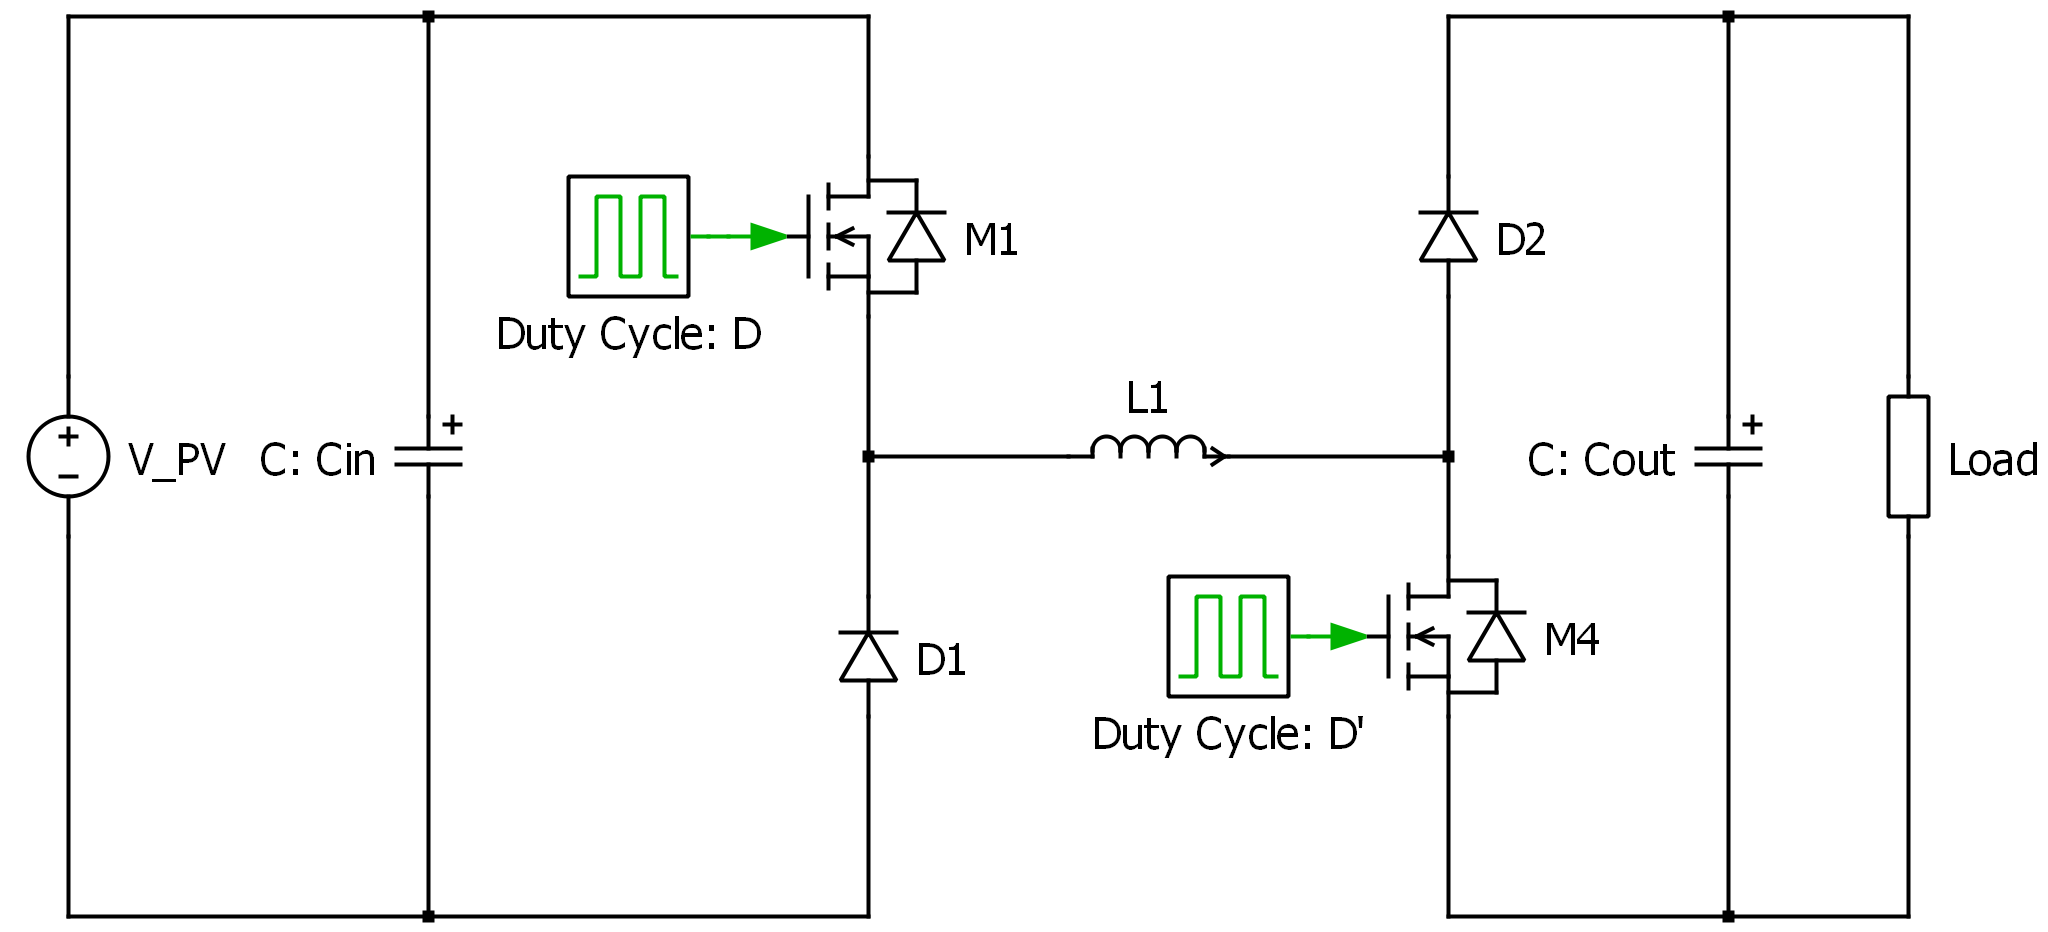
\includegraphics[width=0.8\textwidth]{../Pictures/2_d_H_B_BB}
	\caption{Equivalent circuit for the non-inverting buck-boost converter.}
	\label{N_INV_BB_SCHEMATIC}
	\end{center}	
\end{figure}
	
The controller can force the system to work in any of the following states:

\begin{enumerate}
	\item Buck $\rightarrow$ $ D \subset [0,1];	 D' = 0 $
	\item Boost $\rightarrow$ $ D = 1;	 D' \subset [0,1] $
	\item Buck-Boost $\rightarrow$ $ D \subset [0,1]; D' \subset [0,1] $
\end{enumerate}
		
%Usually, the inverter's input voltage (DC-link voltage) is fixed to some value higher than the peak grid's voltage. 
The possibility of higher and lower voltages at the converter's output allows different ways of associating photovoltaic modules. Then, the user is able to arbitrarily decide how many PV modules to link in series within a range. Differently from what would happen in the case of buck or boost converters where the constraints regarding the number of panels are a bigger concern. In the case of the boost, the number of panels $N$ is limited by the maximum duty cycle that is allowed, following equation \ref{boost_number_of_panels}, where $V_{DC} $ is the voltage at the input of the inverter and $V_{MPP}$ is PV panels' maximum power voltage. In the case of the buck, the number of panels is limited by the minimum allowed duty cycle, as described in equation \ref{buck_number_of_panels}. Then the boost has a more requiring constraint when considering the maximum number of panels and the buck has a more requiring constraint when considering the minimum number of panels.

\begin{equation} \label{boost_number_of_panels}
 N_{min} = \frac{V_{DC} \cdot (1 - D_{max})}{V_{MPP}}
\end{equation}

\begin{equation} \label{buck_number_of_panels}
 N_{max} = \frac{V_{DC}}{V_{MPP} \cdot D_{min}}
\end{equation}

Compared with other topologies that can have both higher and lower voltages at the output, this DC-DC converter features a single inductor and no intermediate capacitor. With such reduction in passive components the price, efficiency and power density improves significantly \cite{underthehood}. One of the drawbacks of the non-inverting buck-boost topology is the control's complexity, which must calculate the appropriate duty cycle $D$ and $D'$ in any of the modes and also the transition between these modes. The buck-boost mode is specially complicated as there are two duty cycles to calculate. This problem might be addressed by setting a constant duty cycle in one of the bridge's legs and then the control will calculate the other leg's duty cycle  \cite{AN4449_ST}.

As seen in figure \ref{BID_N_INV_BB_SCHEMATIC}, the duty cycles of the switches that replace the diodes are $\overline{D}$ and $\overline{D'}$. This line over the variables means that it is the complementary value of the original variable. The duty cycle is the boolean variable that indicates the conduction state of a switch. 
		
Although this topology exhibits appropriate features, it can be further modified by replacing the diodes by MOSFETs. The circuit may be seen in figure \ref{BID_N_INV_BB_SCHEMATIC} and it is called Bidirectional Non-Inverting Buck-Boost converter.

\begin{figure}[H]
	\begin{center}
		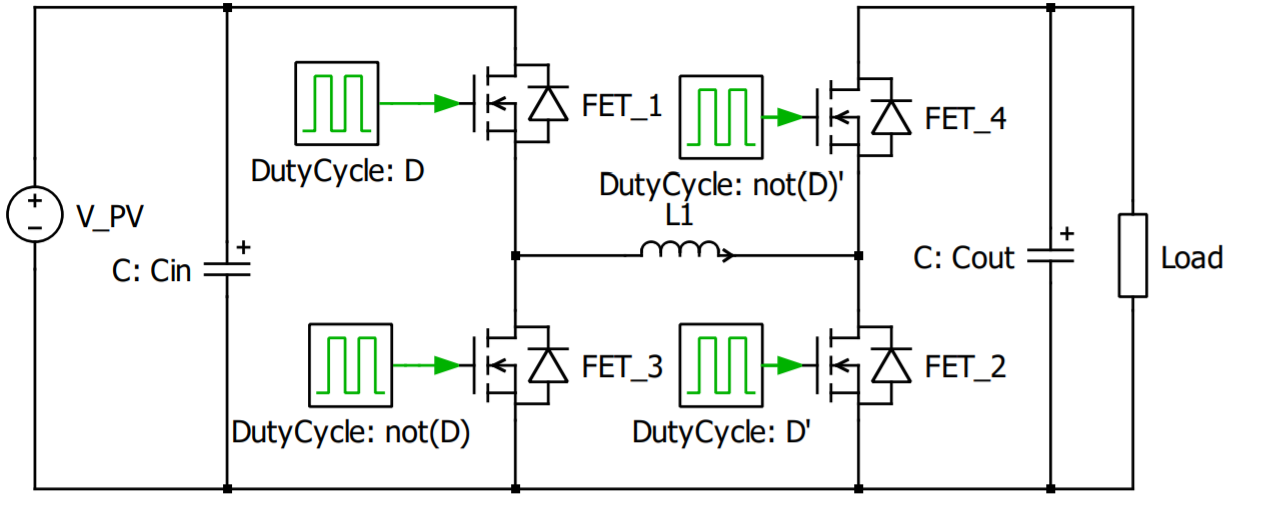
\includegraphics[width=0.8\textwidth]{../Pictures/BID_H_B_BB}
		\caption{Bidirectional Non-inverting buck-boost converter.}
		\label{BID_N_INV_BB_SCHEMATIC}
	\end{center}
\end{figure}

\noindent With this variation, the following changes occur:
		
\begin{enumerate}
	\item The system becomes bidirectional.
	\item The conduction losses are smaller within some current ranges. 
\end{enumerate}

The conduction losses are smaller due to the fact that the losses in a diode evolve with a slope equal to the diode forward voltage: around $0.7V$ for silicon while the losses in a MOSFET evolve quadratically with current with $R_{DS}$, as seen in equations \ref{diode_losses} and \ref{mosfet_losses}. For a $R_{DS}$ of 20 $m\Omega$, the conduction losses will be lower in the MOSFET while the current is below $35 A$. 

\begin{equation}	\label{diode_losses}
	P_{diode} = V_d \cdot I
\end{equation}
	
\begin{equation}	\label{mosfet_losses}
	P_{MOSFET} = I^2 \cdot R_{DS}
\end{equation}


If the system is bidirectional it can be used for different purposes, as the topology seen in figure \ref{BID_MIC_ARCHITECTURES}, which features an isolated DC-link. This topology has a bidirectional MIC, as energy flow in both directions is needed. The goal of this system is to have a single MPP. This is achieved by:

\begin{enumerate}
	\item Set the working conditions to have as many PV  panels performing under the MPP as possible. In this case there are two panels which generate more than the third one.
	\item Now evaluate the power generation difference between those panels working in the MPP and those with a lower power generation. The average power generation is computed.
	\item The control system must lower the power difference to 0. This target is met by getting power from those panels which are generating more than average (in the picture seen as $P_{3}$ and $P_{2}$) and supplying this power back to the panels below the average power generation (in the picture seen as $P_{1}$).
\end{enumerate}

This strategy's advantage is that the power processed by the converters is lower than in a system where all the energy is flowing through the converter. Achieving lower losses, in absolute value. \cite{ArchitectureMIC}

\begin{figure}[H]
	\begin{center}
		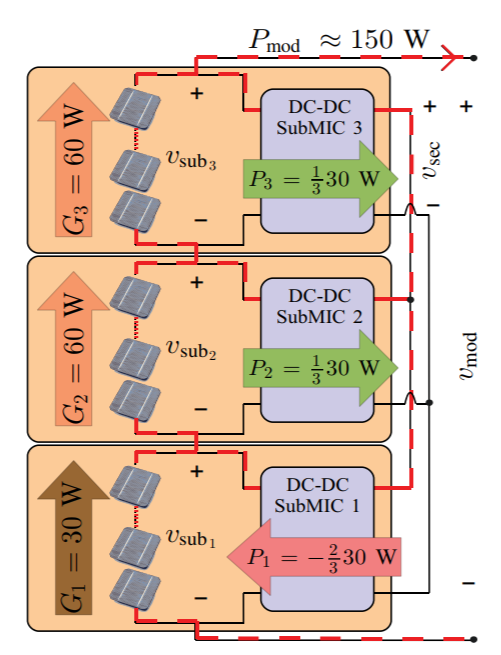
\includegraphics[width=0.4\textwidth]{../Pictures/bidirectional_mic_use}
		\caption{Bidirectional MIC use \cite{ArchitectureMIC}.}
		\label{BID_MIC_ARCHITECTURES}
	\end{center}	
\end{figure}
		
A drawback of the bidirectional system is the increased difficulty of the driver circuitry like the requirement of a dead time in order to avoid the short circuit of $FET_1$ and $FET_3$ or $FET_2$ and $FET_4$, which could damage the system. When using diodes, the system is intrinsically protected against a shoot-through event.
		
